% ============================================================
% A2L-RAGAlign: Calibrated Restoration of Embedded Measurement
%               Interfaces from Firmware Symbols
% Target venue: ISCAS 2027 (regular paper track).  Official requirements: 4
%   pages of body plus an optional 5th page carrying references only; PDF
%   <= 5 MB; all fonts embedded; no Type 3 fonts.  The official LaTeX
%   template is the IEEEtran class in "conference" mode (ISCAS 2027 samples
%   page: "please use the IEEEtran document class file in 'conference'
%   mode"), which is exactly what this file uses -- no separate
%   iscas2027.sty is distributed.  The current build is 5 pages in total:
%   body Sec. I-V spans pages 1-4 exactly; page 5 is the reference list
%   only (both columns).  The production retrieval sweep is reported
%   inline in Sec. IV-E (18.3 -> 25.6 Top-1 points at 83 -> 4,003
%   candidates); tables/tab_production.tex stays in the artifact but is
%   not \input here.
% Design decision (2026-10-25, after the ISCAS review pass): the structural
%   evidence (I/O class + type family) is a *check input*, not a score term.
%   The fusion therefore has two channels with weights 2/3 (retrieval) and 1/3
%   (token); rag_align.W_STRUCTURE is 0.0 and SemanticAligner normalizes the
%   remaining weights.  Rationale and the counterfactual measurement are in
%   Sec. III-C and Table III (row "Ours + struct. score term"): putting the
%   structure back into the score costs 3.5 coverage points and 1.6 points of
%   distractor false positives, changes no ranking result, and removes no
%   false acceptance.  Any change to rag_align.py must be followed by
%   re-running experiments/run_experiments.py, check_results.py and the
%   TikZ/matplotlib figure builders in the same commit.
% Structure:
%   I.    Introduction
%   II.   Related Work
%           A. Embedded Measurement and Configuration Toolchain
%           B. Retrieval-Augmented Software Engineering
%   III.  Methodology
%           A. Problem Setting: The Measurement Contract and Its Drift
%           B. Knowledge Base and Decomposition
%           C. Confidence-Ranked Alignment, Completion, and Consistency
%           D. Implementation
%   IV.   Experiments
%           A. Setup
%           B. Alignment Accuracy on the Firmware-Evolution Workload
%           C. Safety against Contract Violations
%           D. Tiers, Downstream Tasks, and Robustness
%           E. Production-Image Evaluation
%   V.    Conclusion
% Build:  cd paper && _tools\tectonic.exe -X compile main.tex --outdir _build
% Tables: \input from tables/*.tex, all written by
%         experiments/run_experiments.py (do not hand-edit); tab_contract
%         carries the measured detection rates of the drift taxonomy.
% Figures: figures/fig_workflow_compare.pdf (Fig. 1, full width at
%                                            0.72\textwidth: manual vs. tool
%                                            symbol-alignment workflow; the
%                                            single-column overview.pdf was
%                                            dropped for space -- its content
%                                            is stated in Sec. III-B/C)
%          figures/fig_signal_conversion.pdf (Fig. 2, full width at
%                                            0.68\textwidth: per-signal
%                                            engineering walk-through)
%          fig_workflow_compare comes from the TikZ source via
%          paper/figures/build_workflow_compare_figure.py, fig_signal_conversion
%          via paper/figures/build_signal_conversion_figure.py (TeX engine,
%          Type 1 only); every identifier, address, type and score in
%          fig_signal_conversion is reproduced from the artifact (the demo
%          address file data/sample/example.map and the shipped corpus).
%          The figure widths are tuned so that the body stays
%          at four pages: the reference list fills page 5.
%          Rebuild the TikZ source with:
%          py -3.12 paper/figures/build_signal_conversion_figure.py
% Template compliance (IEEEtran V1.8b, conference mode):
%   - \documentclass[conference]{IEEEtran}; the class supplies the two-column
%     Letter layout, the 24 pt title, the Roman-numeral section numbering, the
%     "Abstract--"/"Index Terms--" labels, the "TABLE N" captions above the
%     tables and the "Fig. N." captions below the figures, so none of these
%     are hand-rolled here.
%   - T1 font encoding is requested before \documentclass so IEEEtran's own
%     font selection resolves ptm to the Nimbus Roman (Times) Type 1 fonts
%     instead of falling back to Latin Modern; all fonts end up embedded and
%     no Type 3 font is emitted, as ISCAS requires.
%   - hyperref is loaded last (IEEEtran HOWTO), with hidelinks so the
%     class-styled captions keep no coloured link boxes.
%   - The bibliography keeps IEEEtran's default flow: one continuous list
%     that runs down the left column and continues at the top of the right
%     column, so the reading order is always left -> right.  No \balance:
%     the last page's columns are left unequal on purpose.
% All quoted numbers come from experiments/results/results.json and
% experiments/results/production_alignment.json (regenerate via
% experiments/run_experiments.py and experiments/production_experiment.py).
% ============================================================
% IEEEtran selects the Times family (ptm) for the body text.  Under XeTeX the
% default encoding is TU, where no ptm fonts exist, so the text silently
% falls back to Latin Modern.  The T1 encoding has to be in effect *before*
% the class selects its fonts, so it is requested through a pre-class
% \RequirePackage hook: a \usepackage[T1]{fontenc} placed after
% \documentclass would arrive too late for IEEEtran's own font selection and
% leave the class-init "Font shape TU/ptm undefined" warnings in the log.
% T1 activates the Nimbus Roman (Times) Type 1 fonts, which also matches the
% figures.
\RequirePackage[T1]{fontenc}
\documentclass[conference]{IEEEtran}

% microtype lets TeX shrink/stretch glyph widths by a couple of percent and
% protrude them past the column edge.  Without it a few lines are forced to
% stretch their inter-word spaces far beyond normal, which is visible in the
% two-column layout (and shows up as Underfull \hbox warnings).
\usepackage{microtype}
\usepackage{cite}
\usepackage{amsmath,amssymb,amsfonts}
\usepackage{graphicx}
\usepackage{textcomp}
\usepackage{xcolor}
\usepackage{booktabs}
\usepackage{array}
\usepackage{url}
\usepackage{tikz}
\usetikzlibrary{positioning}
% hyperref must be the last package loaded (IEEEtran HOWTO): it patches the
% caption and bookmark machinery of the class, so any package loaded after it
% can be silently bypassed.  hidelinks keeps the IEEEtran-styled captions
% free of coloured boxes.
\usepackage[hidelinks]{hyperref}

\newcommand{\toolname}{A2L-RAGAlign}
\newcommand{\ie}{\emph{i.e.}}
\newcommand{\eg}{\emph{e.g.}}

\begin{document}

\title{\toolname{}: Calibrated Restoration of Embedded Measurement
Interfaces from Firmware Symbols}

% NOTE ON THE AUTHOR BLOCK.  IEEEtran in conference mode silently discards the
% footnote text produced by \thanks{} (verified: the note never reaches the
% PDF, and \footnotemark/\textsuperscript inside \IEEEauthorblockN breaks
% IEEEtran's math-mode author halign with "Missing $ inserted").  The
% corresponding-author designation is therefore given as a plain line in the
% affiliation block, which renders correctly.
\author{\IEEEauthorblockN{Wei Wang}
\IEEEauthorblockA{East China Normal University\\
Shanghai 200062, China\\
71285902039@stu.ecnu.edu.cn}
\and
\IEEEauthorblockN{Dehui Du}
\IEEEauthorblockA{East China Normal University\\
Shanghai 200062, China\\
dhdu@sei.ecnu.edu.cn\\
Corresponding author}
}

\maketitle

\begin{abstract}
Embedded development of a safety-relevant automotive control unit couples the
firmware to its calibration toolchain through an ASAM MCD-2MC A2L
description file---an executable contract binding every control variable to
its address, raw bit layout, and physical scaling. Every recompilation
invalidates part of that contract, and both restoration
mechanisms---exact string matching and hand-maintained spreadsheets---fail on
ordinary renames. We present \toolname{}, a retrieval-augmented
framework that fuses retrieval and token evidence over an embedded knowledge
base into calibrated alignments, and gates each with a structural contract
check: the I/O class and type family a symbol name carries are compared with
the candidate, and a class or type-family flip---a category error no score can
rank out---is demoted by a penalty and a hard tier cap, so it can never be
auto-accepted. On a held-out split of 314 renamed queries (from 631 generated
over 83 signals) it reaches 99.0\% Top-1 where exact matching scores 0\% and
string similarity 92.4\%, and 97.6\% on the 84 multi-hop renames; on 127
contract-violating pairs it removes false auto-acceptance entirely at 93.6\%
auto-coverage and 99.3\% precision. On the production image itself
(4{,}003 real symbols) it reaches 97.8\% Top-1, and removing the retrieval
channel costs 25.6 Top-1 points.
\end{abstract}

\begin{IEEEkeywords}
A2L, calibration and debug toolchain, contract verification, embedded
measurement interface, firmware evolution, retrieval-augmented alignment
\end{IEEEkeywords}

\section{Introduction}
\label{sec:intro}

An automotive control unit (ECU) is developed, debugged, and calibrated
through a hardware--software toolchain. The target firmware exposes its
internal state over a measurement protocol (XCP~\cite{asam2017xcp}), and a
calibration master (INCA, CANape) reads and writes it through a description
file (MCD-2MC~\cite{asam2018mcd2mc}) stating, for every object, where the
variable lives, how many bits it occupies, which bit range is meaningful, and
how raw counts become physical units. We call this the \emph{embedded
measurement interface}: not documentation but an executable contract---every
bench number is the product of the address, layout, mask, and conversion it
declares.

Firmware evolution breaks that contract continuously. Each recompilation moves
symbols, renames identifiers, changes widths and bit layouts, and adds or
removes variables, so the description must be resynchronized with the binary;
the tool then reads the wrong word, bit range, or class of variable, and the
failure is silent by construction---the master still connects, still plots,
and the engineer sees a plausible value. Restoration today rests on \emph{exact
string matching} and \emph{manually curated spreadsheets}; both break on
ordinary divergence---toolchain-specific spellings, identifier styles
(snake-case \emph{vs.} camel-case, abbreviations \emph{vs.} full
words~\cite{lawrie2006identifiers,binkley2009camelcase}), struct-path
qualification---so engineers fall back to serial lookup.

\begin{figure*}[t]
  \centering
  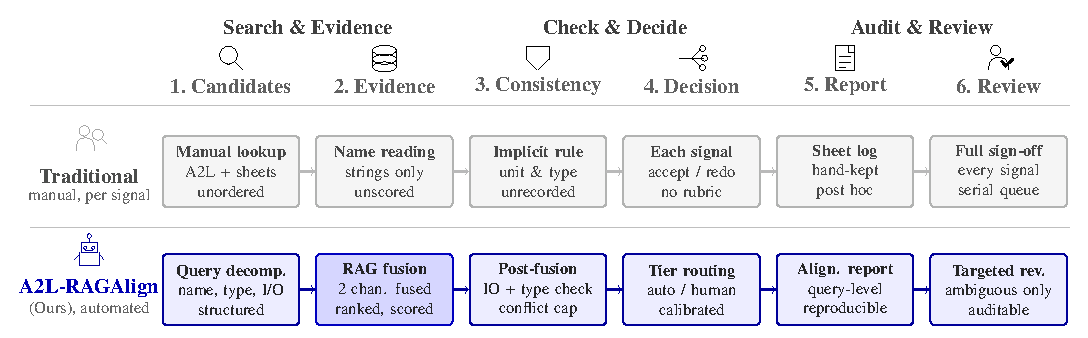
\includegraphics[width=0.72\textwidth]{figures/fig_workflow_compare.pdf}
  \caption{The symbol-alignment workflow, manual versus tool-assisted. The
  manual route is per signal and unrecorded; \toolname{} produces a scored
  candidate, a consistency verdict, and a calibrated decision per query.}
  \label{fig:workflow}
\end{figure*}

Restoring the contract is therefore not a naming problem but a \emph{typed} one,
with the shape of a compiler type check: two objects can agree on every character
of their names and still describe different quantities. The missing ingredient
is \emph{domain knowledge retrieval}: the knowledge to repair a broken
match already exists in an engineering organization---layout rules, naming
conventions, calibration sheets, and the semantic descriptions engineers
attach to signals. \toolname{} packages it as a retrieval-augmented framework
layered on an operational update tool (Fig.~\ref{fig:workflow}), whose tiered
automation delivers the trustworthiness safety-relevant development
demands~\cite{iso26262}.

Our contributions are twofold.
\begin{itemize}
    \item \textbf{Contract-level formalization.} Alignment as evidence
  fusion over an embedded knowledge base, with a per-field \emph{contract
  check} on the two structural fields a name carries (I/O class, type
  family) that hard-caps the two category-level violations: class flip and
  type-family flip (Sec.~\ref{sec:methodology}).
  \item \textbf{Calibrated, auditable automation.} Alignments are tiered
  AUTO/SUGGEST/MANUAL with thresholds calibrated on held-out signals, and
  every decision ships with its evidence in an alignment report, the
  configuration trail the description needs (Sec.~\ref{sec:align}). Ranking
  is near saturation; our contribution is the gate.
\end{itemize}

\section{Related Work}
\label{sec:related}

\subsection{Embedded Measurement and Configuration Toolchain}
\label{sec:rw-infra}
The standards define our path: XCP~\cite{asam2017xcp} the transport,
MCD-2MC~\cite{asam2018mcd2mc} the description, MDF~\cite{asam2025mdf} the master
data, ISO~14229~\cite{iso14229} diagnostic services over the same bus
(CAN~\cite{iso11898}); AUTOSAR~\cite{autosar2018overview} standardizes the
software interfaces, and ELF/DWARF~\cite{dwarf2017dwarf5} is the type truth we
bind to. Existing A2L tooling regenerates the address-bearing part of a
description from the image, while identity and physical metadata remain
hand-carried---costly for safety-relevant software~\cite{iso26262}. Automatic
schema matching~\cite{rahm2001schema} addresses the metadata half---the
abstract twin of our problem---but lacks the structural evidence generic
matchers miss; our baselines follow~\cite{bilenko2003adaptive}.

\subsection{Retrieval-Augmented Software Engineering}
\label{sec:rw-rag}
Surveys chart the rise of LLM-based SE tooling~\cite{fan2023llm4se,hou2024llm4se};
retrieval-augmented generation grounds model outputs in external
knowledge~\cite{lewis2020rag,gao2023ragsurvey}, with dense
retrieval~\cite{karpukhin2020} and code search~\cite{gu2018codesearch} as
substrate; \toolname{} applies the RAG pattern to a configuration artifact,
not source code, and stops short of generation: no language model is called,
so scoring is deterministic and every decision stays auditable.

\section{Methodology}
\label{sec:methodology}

\begin{figure*}[t]
  \centering
  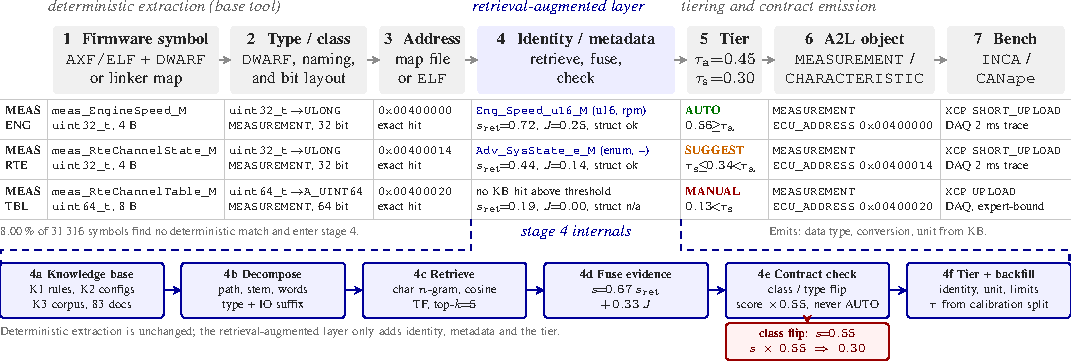
\includegraphics[width=0.68\textwidth]{figures/fig_signal_conversion.pdf}
  \caption{Engineering walk-through on the released demonstration firmware.
  Columns~1--3 are the deterministic chain, column~4 the retrieval-augmented
  layer (stages~4a--4f), and columns~5--7 the tier (calibration-split
  thresholds), the A2L object, and the bench; in the red-boxed class-flip case
  the check multiplies the fused score by 0.55 ($0.55\to0.30$), and the hard
  tier cap keeps a conflicting pair out of AUTO in any case.}
  \label{fig:signal}
\end{figure*}

\subsection{Problem Setting: The Measurement Contract and Its Drift}
\label{sec:motivation}
\textbf{What the contract contains.} The A2L description is the executable
contract of the ECU: its \texttt{MODULE} holds \texttt{MEASUREMENT} and
\texttt{CHARACTERISTIC} objects, each referencing a data type, record layout,
conversion method, and bit mask, with XCP segment definitions tying the
description to the transport~\cite{asam2017xcp}. The base tool derives all of
it from the firmware's ELF/DWARF debug information~\cite{dwarf2017dwarf5},
expanding struct members, arrays, and bitfield masks.

\textbf{Three kinds of drift, and what they cost.} Identity drift renames
variables; schema drift changes type width, bit layout, or class; address
drift moves them at every recompilation. Table~\ref{tab:contract} lists the
resulting error classes. Two are categorical: a name carries \emph{identical}
evidence for a class- or type-flipped twin, so no score can separate them---and
a score that cannot must not auto-accept them.

\begin{table}[t]
\caption{Error taxonomy of a drifted measurement contract, with the measured detection rate of each class and the layer that owns it (Check = alignment contract check, Consist.\ = incremental consistency check).}
\label{tab:contract}
\centering
\scriptsize
\setlength{\tabcolsep}{2pt}
\begin{tabular}{>{\raggedright\arraybackslash}p{1.5cm}
                >{\raggedright\arraybackslash}p{2.2cm}
                >{\raggedright\arraybackslash}p{2.3cm}
                >{\raggedright\arraybackslash}p{1.55cm}}
\toprule
Drift class & At the target & Consequence & Owner \\
\midrule
Class flip & exposed as MEAS & master writes const. & Check (100.0\%) \\
Type-family & layout no longer fits & decodes to another & Check (100.0\%) \\
Bit-layout & mask stops isolating & contaminated $2^{w}-2^{b}$ & Consist.\ (100.0\%) \\
Scaling loss & raw count, wrong $k$ & value off by $6\times$ & Consist.\ (100.0\%) \\
Duplicate & two objects, one var & master reads stale & Consist.\ (100.0\%) \\
Orphan & object vanishes & stale entry kept & Consist.\ (100.0\%) \\
\bottomrule
\end{tabular}
\end{table}


\textbf{Scale.} The problem is not hypothetical: on a production 32-bit ARM
transmission-control image, DWARF extraction yields 31{,}316 signals, of which
exact matching resolves 28{,}812; the remaining 2{,}504 (\textbf{8.00\,\%}) stay
unresolved and are silently dropped---variables that exist in the firmware but
are invisible to the bench. We forensically separated that gap instead of
assuming it: among the 580 distinct names, none survives exact or
case-insensitive lookup in the address file, none appears in the generated
description, and only 9 have even a looser counterpart, so 98.4\,\% are
variables the address file does not export. The 8.00\,\% is a
\emph{symbol-coverage} gap no naming method can close; the naming divergence
alignment \emph{can} absorb is measured on the same image in
Sec.~\ref{sec:prod}.

\subsection{Knowledge Base and Decomposition}
\label{sec:kb}
The knowledge base stores one document per known signal (name, description,
unit, I/O class, C type) from three sources: \textbf{K1} rules---C-type to
A2L type, record-layout, and conversion mappings plus naming-convention
classifiers; \textbf{K2} historical configurations---per-signal annotations
from calibration sheets; \textbf{K3} semantic corpora---names paired with
physical-semantic descriptions. All ship with the artifact, and K2 is
authoritative where they disagree. Each identifier is decomposed into a
struct path, a stem, word tokens (snake- and camel-case boundaries), a type
suffix (\texttt{u8}..\texttt{f64}, \texttt{b}), and an I/O suffix
(\texttt{C} $\rightarrow$ calibration, \texttt{M} $\rightarrow$
measurement)---recovering the contract fields of Table~\ref{tab:contract}
from the name itself.

\subsection{Confidence-Ranked Alignment, Completion, and Consistency}
\label{sec:align}
Given a query symbol, a retriever fetches the top-$k$ knowledge-base
documents ($k{=}5$) through a pluggable protocol: a zero-dependency character
$n$-gram cosine retriever (default and experimental baseline), an optional
sentence-transformer backend~\cite{reimers2019sbert}, and optional FAISS or
Chroma stores behind the same interface; fusion and check are unchanged.
Two evidence channels are fused per candidate:
\begin{equation}
s = w_r \cdot s_{\mathrm{ret}} + w_t \cdot J(\tau_q, \tau_c),
\label{eq:fusion}
\end{equation}
where $s_{\mathrm{ret}}$ is the retrieval score and $J$ the Jaccard overlap of
decomposed tokens~\cite{jaccard1901}. The weights $w_r, w_t$ are positive and
sum to one; the shipped values $(2/3,\,1/3)$ keep $s$ in $[0,1]$ and make the
two channels directly comparable. Exact hits short-circuit to $s{=}1.0$.

\emph{Structural evidence: a check input, not a score term.} The I/O class
and type family the naming convention carries are kept \emph{out} of the
fused score: the two fields fail independently, and an additive encoding lets
one agreement mask the other ($+0.4$ for a class agreement cancels $-0.3$ for
a type conflict), whereas a per-field rule does not.

\emph{Post-fusion contract check.} Lexical and semantic evidence cannot
distinguish a renamed variable from its class- or type-flipped twin: once the
type and I/O suffixes are split off as structural signals, the remaining
evidence is identical, and the mistake is a category error---a measurement
object bound to a calibratable variable lands in the wrong section, and a
wrong type width applies the wrong record layout. The check compares the two
fields against the candidate: on a conflict it multiplies the fused score by
0.55 and \emph{hard-caps} the tier at SUGGEST, so a conflicting alignment can
never be auto-accepted; below $\tau_{\mathrm{s}}$ it lands in MANUAL.

Each result is assigned a tier: \textbf{AUTO} ($s \geq \tau_{\mathrm{a}}$;
no human action), \textbf{SUGGEST} ($s \geq \tau_{\mathrm{s}}$; one-click
confirm), or \textbf{MANUAL}. Thresholds are \emph{not} hand-picked: on a
signal-disjoint calibration split we grid-search $\tau_{\mathrm{a}}$ under
valid-query precision $\geq 98\%$ and distractor false-auto $\leq 5\%$, and
set $\tau_{\mathrm{s}}$ to the largest value keeping AUTO$\cup$SUGGEST
precision $\geq 85\%$: a manual queue may absorb lower precision, an
auto-accept may not. Each run ends with an \emph{alignment report}
(candidate, fused score, per-channel evidence, check flags) and a review
queue; Fig.~\ref{fig:signal} traces the transformation end to end.

The same evidence completes missing metadata (units, descriptions). The
consistency checker compares the signal set against existing A2L names on
four axes: duplicates and type drift are deterministic (against the
knowledge base's historical type), absent objects are flagged as orphans, and
\emph{rename recognition} reports a rename pair, not a removal plus addition.

\subsection{Implementation}
\label{sec:implementation}
\toolname{} extends an operational PyQt5-based A2L update tool ($\sim$7{,}000
lines) with a self-contained prototype module ($\sim$1{,}100 lines) and a thin
adapter ($\sim$160 lines); it passes 360 unit tests and runs on the standard
library alone (optional dense retrievers excepted). A batch entry point slots
into the address-matching stage, so the semantic layer sees exactly the
symbols the deterministic chain missed, both behind an opt-in flag. The
retrieval stage never mutates the regenerated description: candidates are
reported alongside the deterministic ones, and the consistency check compares
written objects against the existing header.

The tool, its embedded knowledge base, and the experiment harness are released
as open source at \url{https://github.com/jack0430-dev/A2L-RAGAlign_2026}.

\section{Experiments}
\label{sec:experiments}

\subsection{Setup}
\label{sec:setup}
\textbf{Corpus and queries.} 83 signals spanning six functional groups
(engine, battery, transmission, vehicle control, HVAC, advanced) of a
transmission-control basic-software set come from the base tool's built-in
demonstration dataset, so the benchmark needs no binary artifacts. Each signal
goes through up to nine renaming transformations (lower-casing, camel-case,
suffix drop, abbreviation and expansion of domain words, struct-path
qualification, I/O token substitution, and two \emph{multi-hop} combinations),
yielding 631 valid queries; 120 further plausible non-existent signals
(distractors) must not be auto-accepted, and 127 class- or type-flipped twins
are demoted to human confirmation.

\textbf{Splits and calibration.} Signals and distractors are split 50/50 into
calibration and test sets; confusables are evaluation-only. The test split
holds 314 queries, 84 of them multi-hop---the hard column of
Table~\ref{tab:align}. Thresholds are calibrated on the calibration split
($\tau_{\mathrm{a}}{=}0.45$, $\tau_{\mathrm{s}}{=}0.30$); reported metrics are
on the test split (with 60 distractors); the shipped defaults are more
conservative ($\tau_{\mathrm{a}}{=}0.85$, $\tau_{\mathrm{s}}{=}0.50$).
Baselines: exact matching, normalized Levenshtein~\cite{levenshtein1966} over
raw names, token-Jaccard over our decomposition, BM25~\cite{robertson2009bm25}
over the same documents, and the $n$-gram retriever alone, all with $k{=}5$.
Control: all non-trivial baselines hold 100\% Top-1 on the 83 unrenamed
signals. Metrics are Top-1/Top-5 and MRR; Table~\ref{tab:safety} reports AUTO
coverage on valid queries (Valid cov.) against false-acceptance rates on
confusable pairs (Conf. FP) and distractors (Distr. FP).

\subsection{Alignment Accuracy on the Firmware-Evolution Workload}
\label{sec:accuracy}
\begin{table}[t]
\caption{Test-split accuracy (N=314 queries, 83 signals; Hard = multi-hop, N=84); the check gates tiering. Retrieval-only and Ours share the identical ranking (the check changes the tier, not the order) and differ in Table~\ref{tab:safety}.}
\label{tab:align}
\centering
\footnotesize
\setlength{\tabcolsep}{3.5pt}
\begin{tabular}{lcccc}
\toprule
Method & Top-1 (\%) & Top-5 (\%) & MRR & Hard Top-1 \\
\midrule
Exact & 0.0 & 0.0 & 0.000 & -- \\
Levenshtein & 92.4 & 98.1 & 0.946 & 78.6 \\
Token-Jaccard & 64.3 & 74.8 & 0.675 & 33.3 \\
BM25 (KB docs) & 96.8 & 100.0 & 0.980 & 95.2 \\
Retrieval-only & 99.0 & 100.0 & 0.994 & 97.6 \\
\textbf{Ours} & \textbf{99.0} & \textbf{100.0} & \textbf{0.994} & \textbf{97.6} \\
\bottomrule
\end{tabular}
\end{table}


Table~\ref{tab:align} shows the main comparison: exact matching scores 0\% by
construction, and Levenshtein degrades on multi-hop renames, where expansion
erases character overlap. Fusion matches the best retrieval and adds the
contract check, holding 100\% Top-1 on seven of the nine transformations,
where the strongest string baseline reaches 78.6\% on the multi-hop subset.
The three residual errors fall in the two abbreviation-heavy transformations
(1 of 7 in \emph{abbrev}, 2 of 42 in \emph{camel\_abbrev}), where the method
only ties the baseline.

\subsection{Safety against Contract Violations}
\label{sec:safety}
\begin{table}[t]
\caption{Safety at auto threshold 0.45: false auto-acceptance on 127 confusable pairs and 60 distractors.}
\label{tab:safety}
\centering
\footnotesize
\setlength{\tabcolsep}{3.5pt}
\begin{tabular}{lccc}
\toprule
Configuration & Valid cov. & Conf.\ FP & Distr.\ FP \\
\midrule
w/o type/IO penalty & 93.9 & 100.0 & 33.3 \\
Ours + struct. score term & 90.1 & 0.0 & 3.3 \\
Retrieval-only & 99.7 & 100.0 & 56.7 \\
Levenshtein & 86.0 & 100.0 & 96.7 \\
\textbf{Ours (full fusion)} & \textbf{93.6} & \textbf{0.0} & \textbf{1.7} \\
\bottomrule
\end{tabular}
\end{table}


Ranking accuracy alone cannot distinguish a safe aligner from an unsafe one.
Table~\ref{tab:safety} therefore evaluates the 127 confusable pairs, where
auto-acceptance is by definition false, against auto coverage. The central
evidence is that the post-fusion check, not the fused score, makes alignment
safe: \emph{every} configuration that drops it---pure retrieval, string
similarity, and fusion without the type/IO penalty---blindly auto-accepts the
flipped twins, whereas the full model eliminates confusable false-acceptance
while giving up 0.3 coverage points against the checkless variant and cutting
the distractor false-positive rate from 33.3\% to 1.7\%. The two channels are
not interchangeable, and an ablation must remove a channel rather than reweight
it: ranking the whole knowledge base by decomposition alone drops Top-1 from
99.0\% to 64.3\% (multi-hop: 97.6\% to 33.3\%), whereas dropping the token
channel leaves the ranking untouched---the retriever already orders candidates
well. The counterfactual row \emph{Ours + struct. score term} puts the
structural evidence back into the score, costing 3.5 coverage points and 1.6
points of distractor false positives and removing no false acceptance---hence
a check input, not a score term.


\subsection{Tiers, Downstream Tasks, and Robustness}
\label{sec:tiers}
With the calibrated thresholds, 93.6\% of the test queries are auto-accepted at
99.3\% precision, 6.1\% require a single confirmation, 0.3\% are fully manual,
and 1 of the 60 held-out distractors would be auto-accepted. Unit completion
transfers the correct unit for 97.8\% of 186 queries; consistency checking
recognizes 100\% of 188 renames and owns the remaining drift classes of
Table~\ref{tab:contract} at 100\% recall, no false orphans. Over 10 random
splits, re-calibrating each time, Top-1 is $99.5{\pm}0.4\%$, hard-subset Top-1
$98.6{\pm}0.9\%$, AUTO coverage $93.5{\pm}1.4\%$ at precision
$99.3{\pm}0.3\%$, and confusable false-acceptance is \emph{zero} in every
split; only the distractor false-positive rate is noisy ($1.8{\pm}2.3\%$), and
the single-split figures above are the default seed.

\textbf{Threats to validity.} The renaming transformations approximate, but do
not exhaust, real-world divergence. The 83-signal corpus covers scalar signals
only, leaving bitfield-packed objects and two-dimensional maps unvalidated.
The production evaluation inherits the image's own coverage: 98.4\,\% of the
unresolved names have no counterpart in the address file, and a looser hit is
not an identity---no renaming method recovers them.

\subsection{Production-Image Evaluation}
\label{sec:prod}
The 83-signal corpus is controlled but small, so we repeat the evaluation on
the released production image: its 4{,}003 address-file symbols---identifier,
I/O class, and width, all the image carries---form the knowledge base, and we
apply the six renaming classes this codebase exhibits (case convention,
camel-case, abbreviation and expansion, member path, multi-hop), 180 sampled
queries per configuration. \toolname{}
reaches 97.8\% Top-1 and 99.4\% Top-5 on the full knowledge base, against
90.6\% for Levenshtein, 88.3\% for BM25, 72.2\% for token-Jaccard, and 0\% for
exact matching. The retrieval sweep answers what the small corpus cannot:
decomposition alone costs 18.3 Top-1 points at 83 candidates, growing to 25.6
at 4{,}003---the deficit grows with the candidate space. Retrieval-augmented
is thus an operational claim, invisible on the small corpus.

\section{Conclusion}
\label{sec:conclusion}
We presented \toolname{}, which restores the embedded measurement interface by
knowledge-grounded fusion under calibrated tiers and a post-fusion contract
check: 99.0\% Top-1 at 93.6\% auto-acceptance (99.3\% precision) on the
held-out split, zero false auto-acceptance on the 127 flipped twins where
retrieval and string similarity fail, and a retrieval channel worth 25.6
Top-1 points on the production image.

% The reference list is inlined (generated once by IEEEtran.bst from
% refs.bib) instead of \bibliography{refs}: two consecutive institutional
% authors (ASAM e.V., ISO) would be typeset as the IEEEtran "------"
% dash, and the venue wants organization names spelled out.  If refs.bib
% changes, regenerate the list with:
%   _tools\tectonic.exe -X compile main.tex --outdir _build --keep-intermediates
% then copy the \bibitem entries from _build\main.bbl back into the
% thebibliography below, and re-apply the two institutional names.
\begin{thebibliography}{10}
\providecommand{\url}[1]{#1}
\csname url@samestyle\endcsname
\providecommand{\newblock}{\relax}
\providecommand{\bibinfo}[2]{#2}
\providecommand{\BIBentrySTDinterwordspacing}{\spaceskip=0pt\relax}
\providecommand{\BIBentryALTinterwordstretchfactor}{4}
\providecommand{\BIBentryALTinterwordspacing}{\spaceskip=\fontdimen2\font plus
\BIBentryALTinterwordstretchfactor\fontdimen3\font minus
  \fontdimen4\font\relax}
\providecommand{\BIBforeignlanguage}[2]{{%
\expandafter\ifx\csname l@#1\endcsname\relax
\typeout{** WARNING: IEEEtran.bst: No hyphenation pattern has been}%
\typeout{** loaded for the language `#1'. Using the pattern for}%
\typeout{** the default language instead.}%
\else
\language=\csname l@#1\endcsname
\fi
#2}}
\providecommand{\BIBdecl}{\relax}
\BIBdecl

\bibitem{asam2017xcp}
\BIBentryALTinterwordspacing
{ASAM e.V.}, ``{ASAM MCD-1 XCP, Version 1.5.0: Universal Measurement and
  Calibration Protocol},'' 2017, {Version} 1.5.0, released 2017-11-30.
  [Online]. Available: \url{https://www.asam.net/standards/detail/mcd-1-xcp/}
\BIBentrySTDinterwordspacing

\bibitem{asam2018mcd2mc}
\BIBentryALTinterwordspacing
{ASAM e.V.}, ``{ASAM MCD-2MC (ASAP2), Version 1.7.1: Data Model for ECU
  Measurement and Calibration},'' 2018, {Version} 1.7.1, released 2018-01-30.
  [Online]. Available: \url{https://www.asam.net/standards/detail/mcd-2-mc/}
\BIBentrySTDinterwordspacing

\bibitem{lawrie2006identifiers}
D.~Lawrie, C.~Morrell, H.~Feild, and D.~Binkley, ``{What's in a Name? A Study
  of Identifiers},'' in \emph{Proc. 14th IEEE International Conference on
  Program Comprehension (ICPC)}, 2006, pp. 3--12.

\bibitem{binkley2009camelcase}
D.~W. Binkley, M.~Davis, D.~J. Lawrie, and C.~Morrell, ``{To CamelCase or
  Under\_Score},'' in \emph{Proc. IEEE International Conference on Program
  Comprehension (ICPC)}, 2009, pp. 158--167.

\bibitem{iso26262}
{International Organization for Standardization}, ``{ISO 26262-1:2018: Road
  Vehicles -- Functional Safety -- Part 1: Vocabulary},'' ISO Standard, 2018,
  edition 2, published 2018-12.

\bibitem{asam2025mdf}
\BIBentryALTinterwordspacing
{ASAM e.V.}, ``{ASAM MDF: Measurement Data Format, Specification of the
  Measurement Data Format Used by Calibration and Analysis Tools},'' 2025,
  {Version} 4.3.0, released 2025-09-23. [Online]. Available:
  \url{https://www.asam.net/standards/detail/mdf/}
\BIBentrySTDinterwordspacing

\bibitem{iso14229}
{International Organization for Standardization}, ``{ISO 14229-1:2026: Road
  Vehicles -- Unified Diagnostic Services (UDS) -- Part 1: Application
  Layer},'' ISO Standard, 2026, edition 4, published 2026-06; supersedes the
  withdrawn ISO 14229-1:2020.

\bibitem{iso11898}
{International Organization for Standardization}, ``{ISO 11898-1:2024: Road
  Vehicles -- Controller Area Network (CAN) -- Part 1: Data Link Layer and
  Physical Coding Sublayer},'' ISO Standard, 2024, edition 3, published
  2024-05; supersedes the withdrawn ISO 11898-1:2015.

\bibitem{autosar2018overview}
\BIBentryALTinterwordspacing
{AUTOSAR Consortium}, ``{AUTOSAR Technical Overview},'' 2018, {Release}
  R4.4.0, released 2018-10-31. [Online]. Available:
  \url{https://www.autosar.org/standards/classic-platform/}
\BIBentrySTDinterwordspacing

\bibitem{dwarf2017dwarf5}
\BIBentryALTinterwordspacing
{DWARF Committee}, ``{DWARF Debugging Information Format, Version 5},'' 2017,
  approved 2017-02-13; DWARF 6 is still a draft. [Online]. Available:
  \url{https://dwarfstd.org/}
\BIBentrySTDinterwordspacing

\bibitem{rahm2001schema}
E.~Rahm and P.~A. Bernstein, ``{A Survey of Approaches to Automatic Schema
  Matching},'' \emph{The VLDB Journal}, vol.~10, no.~4, pp. 334--350, 2001.

\bibitem{bilenko2003adaptive}
M.~Bilenko, R.~Mooney, W.~Cohen, P.~Ravikumar, and S.~Fienberg, ``{Adaptive
  Name Matching in Information Integration},'' \emph{IEEE Intelligent
  Systems}, vol.~18, no.~5, pp. 16--23, 2003.

\bibitem{fan2023llm4se}
A.~Fan \emph{et~al.}, ``{Large Language Models for Software Engineering:
  Survey and Open Problems},'' in \emph{Proc. IEEE/ACM International
  Conference on Software Engineering: Future of Software Engineering
  (ICSE-FoSE)}, 2023, pp. 31--53.

\bibitem{hou2024llm4se}
X.~Hou \emph{et~al.}, ``{Large Language Models for Software Engineering: A
  Systematic Literature Review},'' \emph{ACM Transactions on Software
  Engineering and Methodology (TOSEM)}, vol.~33, no.~8, pp. 1--79, 2024.

\bibitem{lewis2020rag}
P.~Lewis \emph{et~al.}, ``{Retrieval-Augmented Generation for
  Knowledge-Intensive {NLP} Tasks},'' in \emph{Advances in Neural Information
  Processing Systems (NeurIPS)}, vol.~33.\hskip 1em plus 0.5em minus
  0.4em\relax Curran Associates, Inc., 2020, pp. 9459--9474.

\bibitem{gao2023ragsurvey}
\BIBentryALTinterwordspacing
Y.~Gao \emph{et~al.}, ``{Retrieval-Augmented Generation for Large Language
  Models: A Survey},'' \emph{arXiv preprint arXiv:2312.10997}, 2023. [Online].
  Available: \url{https://arxiv.org/abs/2312.10997}
\BIBentrySTDinterwordspacing

\bibitem{karpukhin2020}
\BIBentryALTinterwordspacing
V.~Karpukhin \emph{et~al.}, ``{Dense Passage Retrieval for Open-Domain
  Question Answering},'' in \emph{Proc. 2020 Conference on Empirical Methods
  in Natural Language Processing (EMNLP)}.\hskip 1em plus 0.5em minus
  0.4em\relax Association for Computational Linguistics, 2020, pp. 6769--6781.
  [Online]. Available: \url{https://aclanthology.org/2020.emnlp-main.550/}
\BIBentrySTDinterwordspacing

\bibitem{gu2018codesearch}
X.~Gu, H.~Zhang, and S.~Kim, ``{Deep Code Search},'' in \emph{Proc. 40th
  ACM/IEEE International Conference on Software Engineering (ICSE)}, 2018,
  pp. 933--944.

\bibitem{reimers2019sbert}
\BIBentryALTinterwordspacing
N.~Reimers and I.~Gurevych, ``{Sentence-BERT: Sentence Embeddings using
  Siamese BERT-Networks},'' in \emph{Proc. 2019 Conference on Empirical
  Methods in Natural Language Processing and the 9th International Joint
  Conference on Natural Language Processing (EMNLP-IJCNLP)}.\hskip 1em plus
  0.5em minus 0.4em\relax Association for Computational Linguistics, 2019,
  pp. 3982--3992.  [Online]. Available: \url{https://aclanthology.org/D19-1410/}
\BIBentrySTDinterwordspacing

\bibitem{jaccard1901}
P.~Jaccard, ``{\'E}tude comparative de la distribution florale dans une portion
  des {Alpes} et du {Jura},'' \emph{Bulletin de la Soci{\'e}t{\'e} Vaudoise des
  Sciences Naturelles}, vol.~37, pp. 547--579, 1901.

\bibitem{levenshtein1966}
V.~I. Levenshtein, ``{Binary Codes Capable of Correcting Deletions, Insertions,
  and Reversals},'' \emph{Soviet Physics Doklady}, vol.~10, no.~8, pp.
  707--710, 1966.

\bibitem{robertson2009bm25}
S.~Robertson and H.~Zaragoza, ``{The Probabilistic Relevance Framework: {BM25}
  and Beyond},'' \emph{Foundations and Trends in Information Retrieval},
  vol.~3, no.~4, pp. 333--389, 2009.

\end{thebibliography}

\end{document}
